\textbf{\textit{Ingwersen}}\autocite{Ingwersen} claims that the in-domain model \hyperref[sec:Places365]{Places365} has a huge advantage over the general-domain model \hyperref[sec:ImageNet]{ImageNet}. As shown in \hyperref[Improvement]{Previous Work and improvements}, this was built on the wrong assumptions, because the baseline accuracies were misleading. The new knowledge obtained about the true baseline accuracies in \hyperref[Improvement]{Previous Work and improvements} prepares the ground for achieving the goal described in \hyperref[sec:Problem Definition]{Problem Definition}. It is in this section it is investigated if it is true that the in-domain model does indeed have the huge advantage claimed in previous study by \textbf{\textit{Ingwersen}}. Or if it is possible to fine tune a general-domain model to perform equally as well as the in-domain model. To do this the general-domain model were trained according to the method described in: \hyperref[methodTransferlearning]{Transfer Learning}.
\subsection{Transfer Learning}
\subsubsection{ResNet50}
Through the early stages of the project, it was really difficult to get any notable improvements to the ResNet50 model. Only small improvements could be seen on the top-1 accuracy, which went from 32\% to 35\% after training with the revised dataset for 20 hours, after the bug was found in the preprocessing scheme, the top-1 accuracy went from 35\% to 65.5\%. This seemed to be a huge improvement, and because a proper baseline were found, the actual transfer learning could begin. As suggested in \textbf{\textit{Ingwersen}} the preprocessing scheme should have a huge impact on scoring better top-1 accuracies, and especially the places preprocessing scheme should be the better choice, as per: \hyperref[appendix: A]{Appendix: A}. To get the most accurate results different layers were trained, and what seemed to be most accurate to train were to train the entire stage 5, as per \hyperref[appendix: C]{Appendix: C}:
\begin{table}[H]
  \centering
\begin{tabular}{llll}
Model\textbackslash{}Processing Scheme & Places365                        & ResNet50                                          & EfficientNet                  \\ \hline
\multicolumn{1}{|l|}{Resnet50}         & \multicolumn{1}{l|}{0.522673} & \multicolumn{1}{l|}{\underline{0.773270}}                     & \multicolumn{1}{l|}{0.662689} \\ \hline
\end{tabular}
\caption{Top-1 accuracies for the ResNet50, w.r. to different preprocessing schemes.}
\end{table}
In the above table, the best performing top-1 accuracy for the ResNet50 model, with stage 5 fine-tuned, is the version trained on the ResNet50 preprocessing scheme.
\subsubsection{EfficientNetB0}
The EfficientNet model, which is a more compact and complicated model compared to the ResNet50, have been investigated. This was done because the feature vector it produces is smaller, and it was believed to be able to represent the rooms at least equally as well as the ReNet50 model, because it was proved to performing a better on the ImageNet test set in \autocite{tan2020efficientnet}. To get the best optimal number of layers trained, different layers were investigated. Below is the top-1 accuracy across layers trained:
\begin{table}[H]
\begin{tabular}{ll}
Trainable layer       & Top-1 Accuracy                       \\
Entire stage 7                          & 76\%                    \\ \cline{2-2}
\multicolumn{1}{l|}{Entire Stage 7, and Stage 6 (D,C)} & \multicolumn{1}{l|}{77,6\%} \\ \cline{2-2}
Entire Stage 7 and entire Stage 6                 & 71\%
\end{tabular}
\caption{EfficientNetB0 trained with different with different layers.}
\end{table}
Different preprocessing schemes were also investigated, to see how well each performed on this model:
\begin{table}[H]
  \centering
\begin{tabular}{llll}
Model\textbackslash{}Processing Scheme & Places                        & Resnet50                                          & EfficientNet                  \\ \hline
\multicolumn{1}{|l|}{EffecientNet}     & \multicolumn{1}{l|}{0.735879} & \multicolumn{1}{l|}{0.731901} & \multicolumn{1}{l|}{\underline{0.776452}} \\ \hline
\end{tabular}
\caption{EfficientNetB0 trained with different preprocessing schemes.}
\end{table}
In the table above, the best performing top-1 accuracy for the EffecientNet model, with the entire stage 7 and stage 6 (D,C) fine-tuned, is the version trained on the EfficientNet preprocessing scheme.
\subsubsection{Comparison to Gold Standard}
The above results should be compared to the \hyperref[goldstandard]{Gold Standard}. \textbf{\textit{Ingwersen}} managed to achieve a top-1 accuracy of 78.3\%, which was a 2.3\% increase compared to baseline model in his study. The best model in \textbf{\textit{Ingwersen}} were obtained by mapping the in-domain model to a 512 dimensional vector. The gap between the baselines obtained in this study and the \hyperref[goldstandard]{Gold Standard}:
\begin{table}[H]
\centering
\begin{tabular}{lll}
Model     & Baseline top-1 Accuracy                      & Gap to Gold standard     \\ \hline
\multicolumn{1}{|l|}{EffecientNet} & \multicolumn{1}{l|}{0.719968} & \multicolumn{1}{l|}{6.3\% points} \\ \hline
\multicolumn{1}{|l|}{ResNet50}     & \multicolumn{1}{l|}{0.655529} & \multicolumn{1}{l|}{12.3\% points}       \\ \hline
\end{tabular}
\caption{Top-1 accuracy of Baseline, and their gap to the Gold Standard.}
\end{table}
The best performing transfer learned model for each general purpose CNN is reported below, together with their gap to the Gold Standard:
\begin{table}[H]
\centering
\begin{tabular}{llll}
Model     & Top-1 Accuracy      & Gap to Gold standard & Improvement     \\ \hline
\multicolumn{1}{|l|}{Effecientnet} & \multicolumn{1}{l|}{0.776452} & \multicolumn{1}{l|}{0.7\% points} & \multicolumn{1}{l|}{5.6\% points} \\ \hline
\multicolumn{1}{|l|}{Resnet50}     & \multicolumn{1}{l|}{0.773270} & \multicolumn{1}{l|}{1\% points}  &   \multicolumn{1}{l|}{11.3\% points}  \\ \hline
\end{tabular}
\caption{Top-1 accuracy of the best performing transfer learned models, and their gap to the Gold Standard, the improvement from the baseline is also reported. }
\end{table}
The best performing transfer learned ResNet50 model had a large gap to the \textbf{Gold Standard}, through transfer learning the gap was almost closed, however if this result is compared to in-domain model with the same feature vector dimension, the two models perform equal. The in-domain 2048 model also have a top-1 accuracy of 77.3\% as reported in \hyperref[appendix: B]{Appendix: B}. The best performing transfer learned EfficientNetB0 model had a smaller gap to the \textbf{Gold Standard} and almost closed the gap, 0.7\% off. It should be taken into account that the feature vector of the EfficientNetB0 model had dimensions of 1280 while \textbf{Gold Standard} had dimensions of 512.
\subsection{Contrastive Learning}
Contrastive learning was applied to the general-domain model, as an attempt to close the gap even further. The reference code, which the contrastive model of this project were built on is located at: https://github.com/wangz10/contrastive\_loss, however due to the different experiment setup, i.e. small batch size compared to \textbf{\textit{Khosla}}\autocite{khosla2020supervised}, and because the goal of this study was to close the gap between an in-domain model and the general-domain model, the contrastive learning needed to be applied to the pre-trained general-domain network, which is not the case in \textbf{\textit{Khosla}}, \textbf{\textit{Khosla}} trained their network from the bottom and up, this was not possible in this study, due to the limited dataset. This led to problems, which caused the loss to update all weights in the network to "NaN"s halfway through training. Below is the loss measurements, which show the loss being minimised for the first 30 epochs, after this no loss could be reported.

\begin{figure}[H]
    \centering
    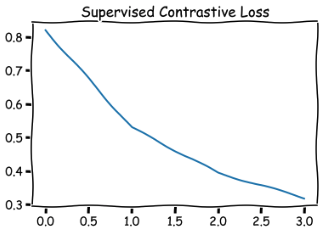
\includegraphics[width =0.4\textwidth]{pictures/random/supconlossfail}
    \caption{The loss of the network seems to be minimised for the first 30 epochs. After this no loss were reported, and all the weights were changed to "NaN".}
    \label{ref:supconlossfail}
\end{figure}
The screenshot of the reported loss value are reported below:
\begin{figure}[H]
    \centering
    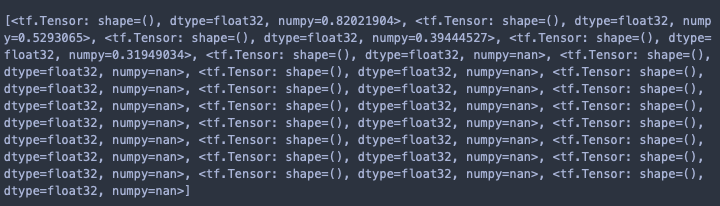
\includegraphics[width =0.90\textwidth]{pictures/random/supconlosserror}
    \caption{The first 30 epochs seems to work fine. But then "NaN" error occurs.}
    \label{ref:supconlosserror}
\end{figure}
Unfortunately it was not possible to recover the weights before the model broke, and no top-1 accuracy could be measured. However as the \hyperref[ref:supconlossfail]{loss measurements} show, it seems to be working, and progressing well, which suggest that the idea might be worth to implement. The failure of the contrastive learned model is further described in \hyperref[sec:Conclusion]{Conclusion}.

\subsection{Show Case: How well does the models predict similar rooms?}
The plots below show how well the two general domain models are able to produce meaningful representations of features in rooms. For full size image plots go to \hyperref[appendix: D]{Appendix: D}.
\subsubsection{ResNet50}
\begin{figure}[H]
    \centering
    \begin{subfigure}[b]{0.45\textwidth}
      \centering
      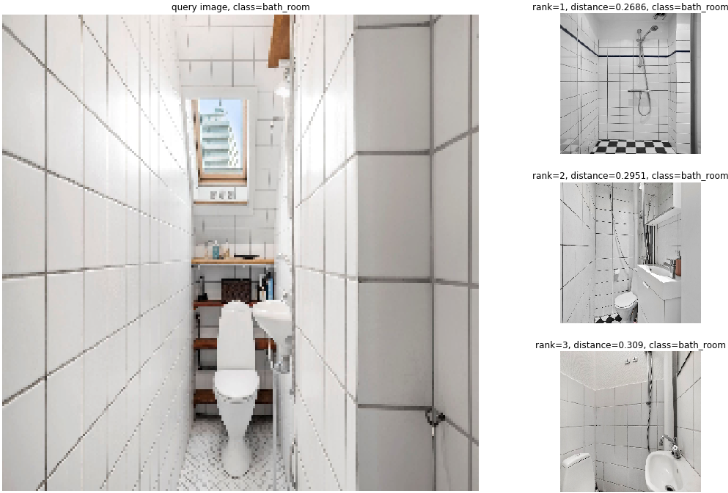
\includegraphics[width=\textwidth]{pictures/random/resnet50bathroomplot}
      \label{fig:1}
    \end{subfigure}
    \hfill
    \begin{subfigure}[b]{0.45\textwidth}
      \centering
      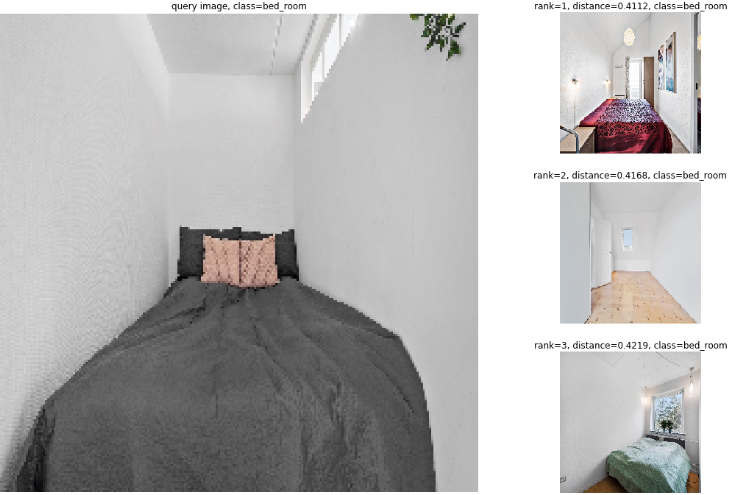
\includegraphics[width=\textwidth]{pictures/random/resnet50bedroomplot}
      \label{fig:2}
    \end{subfigure}
    \hfill
    \begin{subfigure}[b]{0.45\textwidth}
      \centering
      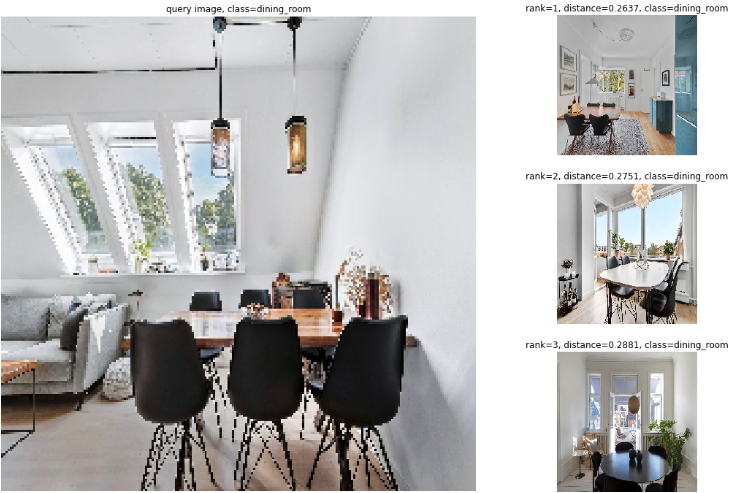
\includegraphics[width=\textwidth]{pictures/random/resnet50diningplot}
      \label{fig:3}
    \end{subfigure}
    \hfill
    \begin{subfigure}[b]{0.45\textwidth}
      \centering
      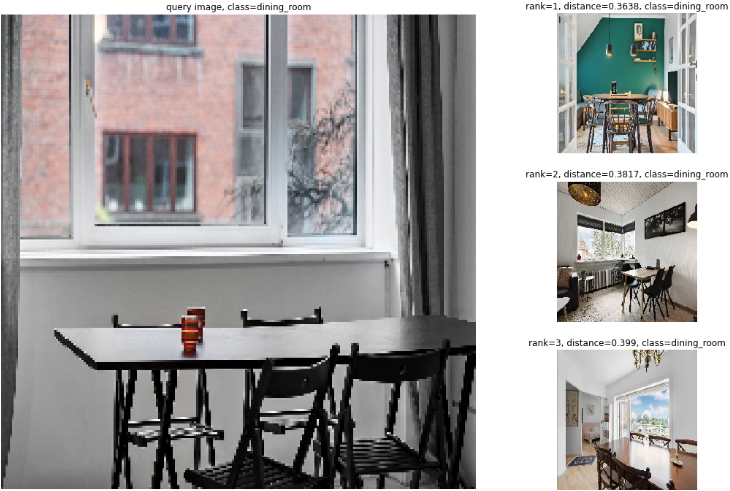
\includegraphics[width=\textwidth]{pictures/random/resnet50diningplot1}
      \label{fig:4}
    \end{subfigure}
    \caption{ResNet50, prediction of the 3 most similar rooms}
    \label{fig:misfoster}
\end{figure}
The ResNet50 model have a top-1 accuracy of 77.3\%, and are able to capture key features in rooms as seen in the above plotted images. The first case, the model is able to capture the distinctive tiles which decorates the walls of the bathroom. In the second case, bedroom, the model is able to capture the size of the room. Home seekers who are looking for homes, which do not use excessive space on the bedrooms, will be able to mark this as a preferred aesthetic preference to get homes that matches that criterion. Same thing goes for the tiles in the bathroom.
\subsubsection{EffecientNet}
\begin{figure}[H]
    \centering
    \begin{subfigure}[b]{0.45\textwidth}
      \centering
      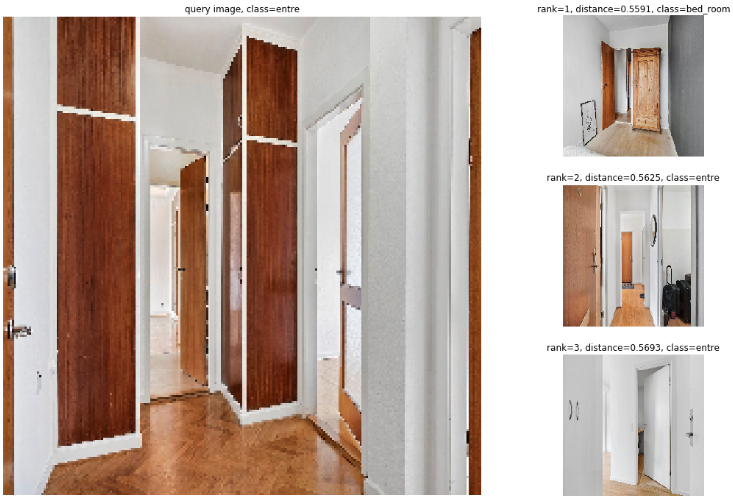
\includegraphics[width=\textwidth]{pictures/random/efnentreplot}
      \label{fig:1}
    \end{subfigure}
    \hfill
    \begin{subfigure}[b]{0.45\textwidth}
      \centering
      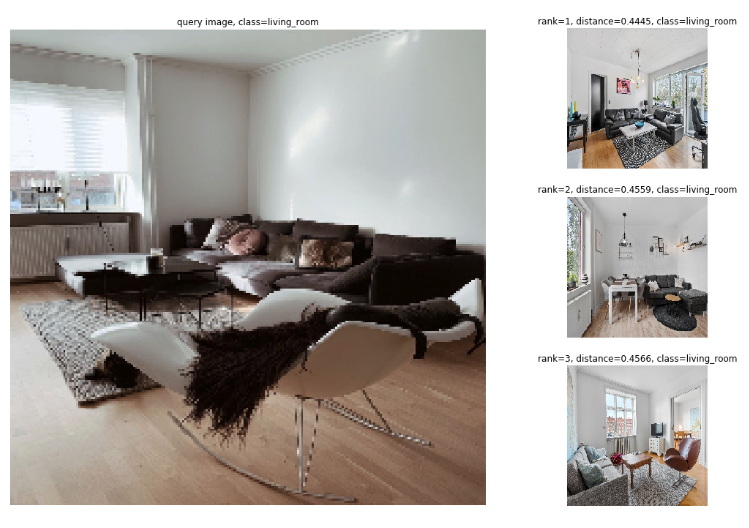
\includegraphics[width=\textwidth]{pictures/random/efnlivingplot}
      \label{fig:2}
    \end{subfigure}
    \hfill
    \begin{subfigure}[b]{0.45\textwidth}
      \centering
      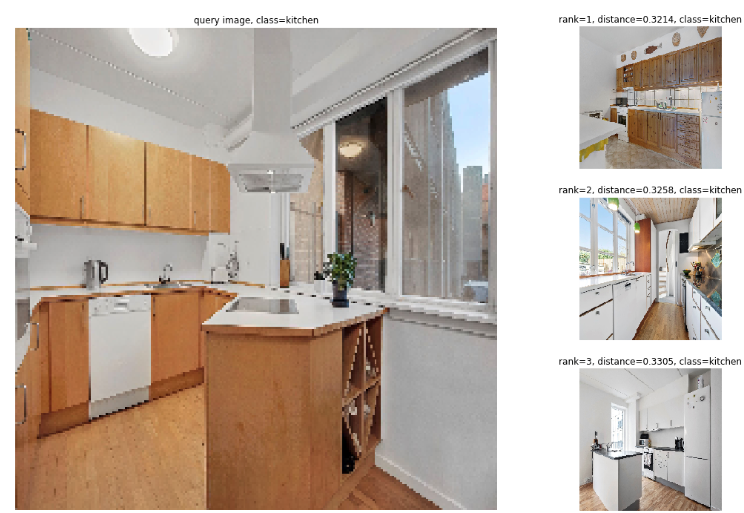
\includegraphics[width=\textwidth]{pictures/random/efnkitchenplot}
      \label{fig:3}
    \end{subfigure}
    \hfill
    \begin{subfigure}[b]{0.45\textwidth}
      \centering
      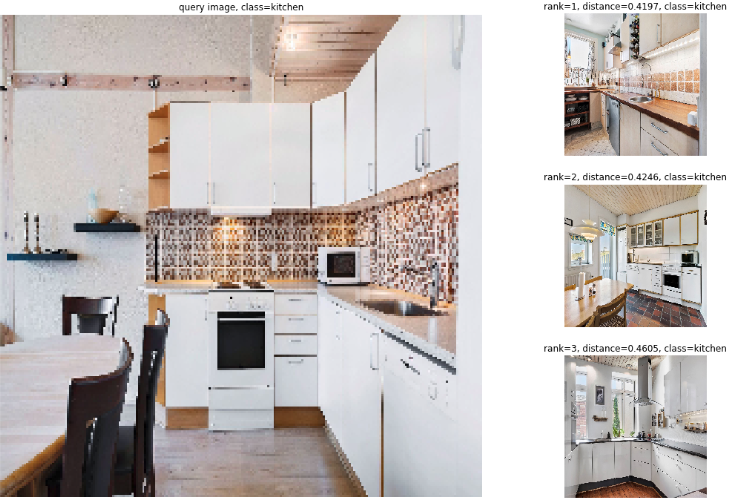
\includegraphics[width=\textwidth]{pictures/random/efnkitchenplot1}
      \label{fig:4}
    \end{subfigure}
    \caption{EfficientNetB0, prediction of the 3 most similar rooms}
    \label{fig:misfoster}
\end{figure}
The EffecientNet model have a top-1 accuracy of 77.6\%, and are also able to produce meaningful representations of the rooms. These images, show a few interesting results as well. The first case, a bedroom is matched as being the nearest room to the entre, and by looking at the images, it is clear that the model has caught the use of wooden materials. The first kitchen case also showcase the ability to capture wooden materials used in the kitchen, while the second kitchen case has caught the use of retro tiles on the walls and floor of the kitchens.

\subsubsection{Untrained ResNet50}
\begin{figure}[H]
    \centering
    \begin{subfigure}[b]{0.45\textwidth}
      \centering
      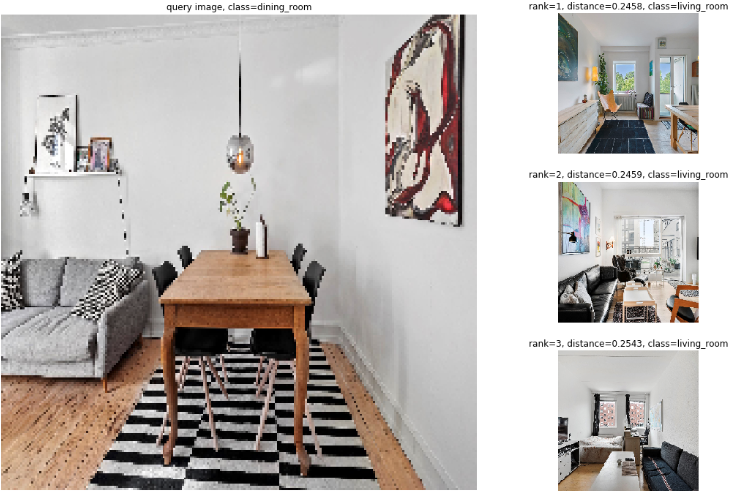
\includegraphics[width=\textwidth]{pictures/random/untrainedkitchenplot}
      \label{fig:1}
    \end{subfigure}
    \hfill
    \begin{subfigure}[b]{0.45\textwidth}
      \centering
      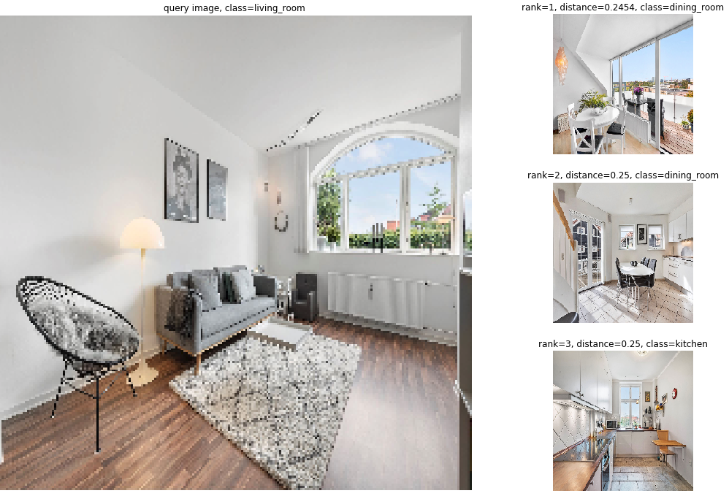
\includegraphics[width=\textwidth]{pictures/random/untrainedlivingroom}
      \label{fig:2}
    \end{subfigure}
    \caption{The untrained model, not capturing alot of the key features, like rugs and windows. Also predicts wrong room label.}
\end{figure}
Above is the untrained model showcased, which have a top-1 accuracy of 65.6\%, to establish if the transfer learning has proved to be a success. The images tells the story that the untrained model is not performing equally as well as the transfer learned models, on the sole argument that it is not capturing the right labels for the classes. The model also does not capture the key features of the rooms, like the lack of windows in the first living room image, and also not venetian style window in the second living room image.
